% !TeX program = lualatex
% !TeX encoding = utf8
% !TeX spellcheck = uk_UA

\documentclass[]{beamer}
\usetheme{PlasmaPhysics}
\usepackage{PlasmaPhysics}
\usetikzlibrary{shadings}
\graphicspath{{pictures}}

%\NewDocumentCommand{\E}{}{\vec{E}}
%\NewDocumentCommand{\B}{}{\vec{B}}
%\NewDocumentCommand{\J}{}{\vec{j}}
%\NewDocumentCommand{\V}{}{\vec{v}}
%\NewDocumentCommand{\wk}{}{\vec{k}}
%
%\NewDocumentCommand{\divg}{m}{\vec{\nabla}\cdot{#1}}
%\NewDocumentCommand{\rot}{m}{\vec{\nabla}\times{#1}}
%\NewDocumentCommand{\grad}{m}{\vec{\nabla}#1}
%\NewDocumentCommand{\vecdot}{mm}{\left[#1\times#2\right]}
%\NewDocumentCommand{\scdot}{mm}{\left(#1\cdot#2\right)}
%\NewDocumentCommand{\dt}{m}{\frac{\partial #1}{\partial t}}
%\NewDocumentCommand{\ddt}{m}{\frac{\partial^2 #1}{\partial t^2}}

\usepackage{subcaption}
\usepackage{mathtools}
\setlength{\abovedisplayskip}{3pt}
\setlength{\belowdisplayskip}{3pt}
\usetikzlibrary{decorations.pathreplacing}
\newtcolorbox{mysidebyside}[1][]{
    notitle, sidebyside, blanker,
    sidebyside align=center seam,
    halign=center,
    lefthand width=.5\textwidth,
    #1
}



\graphicspath{{pictures/}}
\title[Лекції з фізики плазми]{\bfseries\huge Стійкість магнітогідродинамічних конфігурацій}
\subtitle{\bfseries Лекції з фізики плазми}
\author{Пономаренко С. М.}
\date{}
% https://www.youtube.com/watch?v=zv9Y7YmHyBk
\def\stext#1{\text{
        \makebox[0pt]{
            \tikz[baseline] {\node[text width=50pt, align=center, execute at begin node=\setlength{\baselineskip}{-0.5ex}, blue] {#1};}
        }
}}

\begin{document}

% --- Слайд 1 ---
\begin{frame}
	\titlepage
\end{frame}



% --- Слайд 2: Вступ ---
\begin{frame}{Проблема стійкості рівноваги}{}
	\begin{block}{Рівноважний стан}\justifying
		У попередніх розділах ми встановили умови МГД-рівноваги:
		\begin{equation*}
			\grad p_0 = \frac{1}{c} \vecdot{\J_0}{\B_0}
		\end{equation*}
		Проте рівновага може бути як стійкою, так і нестійкою. У плазмових пастках нестійкості призводять до руйнування конфігурації за часи порядка мікросекунд.
	\end{block}
	\begin{alertblock}{Мета лекції}\centering
		Дослідити умови, за яких малі збурення рівноважних величин починають необмежено зростати.
	\end{alertblock}
\end{frame}

% --- Слайд 3: Рівняння для збурень ---
\begin{frame}{Математичне формулювання}{}
	\begin{block}{Лінеаризація рівнянь}\justifying
		За аналогією з теорією хвиль, розглянемо мале зміщення $\vec{\xi}$.
		\begin{equation*}
			\rho_0 \ddt{\vec{\xi}} = -\grad p_1 + \frac{1}{c} \left( \vecdot{\J_1}{\B_0} + \vecdot{\J_0}{\B_1} \right)
		\end{equation*}
	\end{block}
	\begin{block}{Метод нормальних мод}\justifying
		Шукаємо розв'язок у вигляді $\vec{\xi} \sim \exp(-i\omega t)$. Тоді оператор $\ddt{}$ перетворюється на $-\omega^2$:
		\begin{equation*}
			-\omega^2 \rho_0 \vec{\xi} = \vec{F}(\vec{\xi})
		\end{equation*}
		де $\vec{F}(\vec{\xi})$ --- сукупність магнітних та газокінетичних сил, що виникають при зміщенні.
	\end{block}
\end{frame}

% --- Слайд 4: Критерій нестійкості ---
\begin{frame}{Критерій нестійкості}{}
	Аналіз власного значення $\omega^2$ дозволяє визначити долю збурення:
	\begin{itemize}
		\item \textbf{$\omega^2 > 0$} --- частота $\omega$ дійсна. Збурення коливається навколо точки рівноваги. Це відповідає \alert{МГД-хвилям}.
		\item \textbf{$\omega^2 < 0$} --- частота уявна $\omega = i\gamma$. Збурення зростає експоненціально:
		\begin{equation*}
			\vec{\xi} \sim e^{\gamma t}, \quad \gamma = \sqrt{-\omega^2}
		\end{equation*}
		Система \alert{нестійка}. Сила $\vec{F}(\vec{\xi})$ спрямована в бік зміщення.
	\end{itemize}
\end{frame}

% --- Слайд 5: Геометрія в циліндрі ---
\begin{frame}{Збурення в циліндричній геометрії}{}
	Для плазмового шнура розкладаємо зміщення за гармоніками (модами):
	\begin{equation*}
		\vec{\xi}(r, \phi, z) = \vec{\xi}(r) \exp[i(m\phi + kz)]
	\end{equation*}
	\begin{itemize}
		\item $m$ --- азимутальне число, що визначає симетрію перерізу.
		\item $k$ --- поздовжнє хвильове число.
	\end{itemize}

\end{frame}

% --- Слайд 6: Перетяжка m=0 ---
\begin{frame}{Нестійкість перетяжки ($m=0$)}{}
	\begin{block}{Фізика процесу}\justifying
		Розглянемо $Z$-пінч з поверхневим струмом. Магнітний тиск на поверхні (див. \textit{Задачу 3}): $P_{mag} = \frac{B_\phi^2}{8\pi} = \frac{I^2}{2\pi c^2 r^2}$.
	\end{block}
	\begin{itemize}
		\item При випадковому звуженні $\delta r < 0$ магнітний тиск зростає як $1/r^2$.
		\item Якщо магнітний тиск зростає швидше за газовий, шнур продовжує стискатися до повного розриву.
	\end{itemize}

%---------------------------------------------------------
\begin{center}
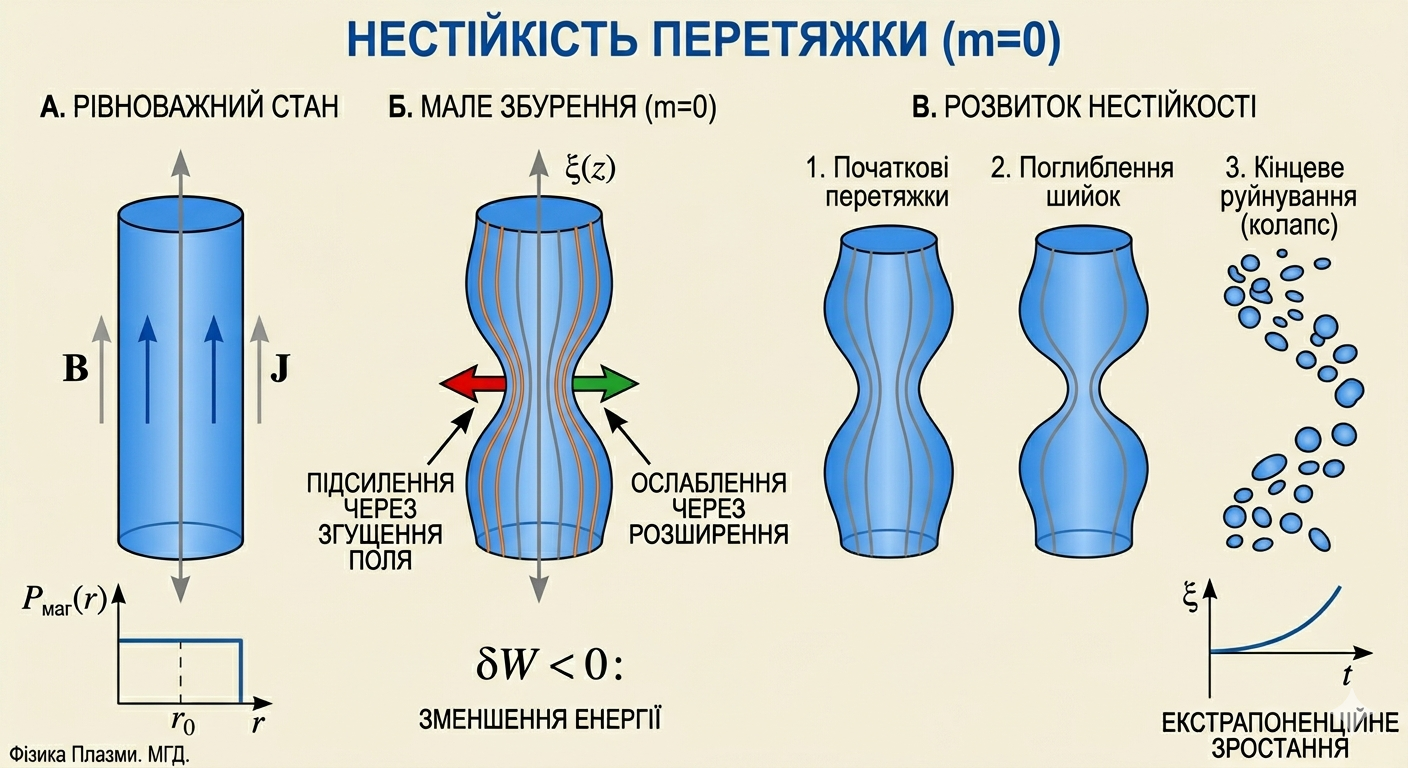
\includegraphics[width=0.75\linewidth]{pic/m0_instab.png}
\end{center}
%---------------------------------------------------------

%	\textit{\scriptsize Перетяжка виникає, коли енергія магнітного поля зменшується при стисненні.}

\end{frame}

% --- Слайд 7: Згин m=1 ---
\begin{frame}{Гвинтова нестійкість (згин, $m=1$)}{}
	\begin{columns}[t]
		\begin{column}{0.5\linewidth}
			\begin{block}{Механізм}\justifying
				При вигині шнура густина силових ліній $B_\phi$ стає більшою на внутрішній стороні вигину.
				Надлишок магнітного тиску виштовхує плазму ще далі.
			\end{block}
		\end{column}
		\begin{column}{0.5\linewidth}
			\begin{alertblock}{Наслідок}
				Це призводить до швидкого викиду плазми на стінки. У токамаках це головна причина зривів.
			\end{alertblock}
		\end{column}
	\end{columns}
%---------------------------------------------------------
\begin{center}
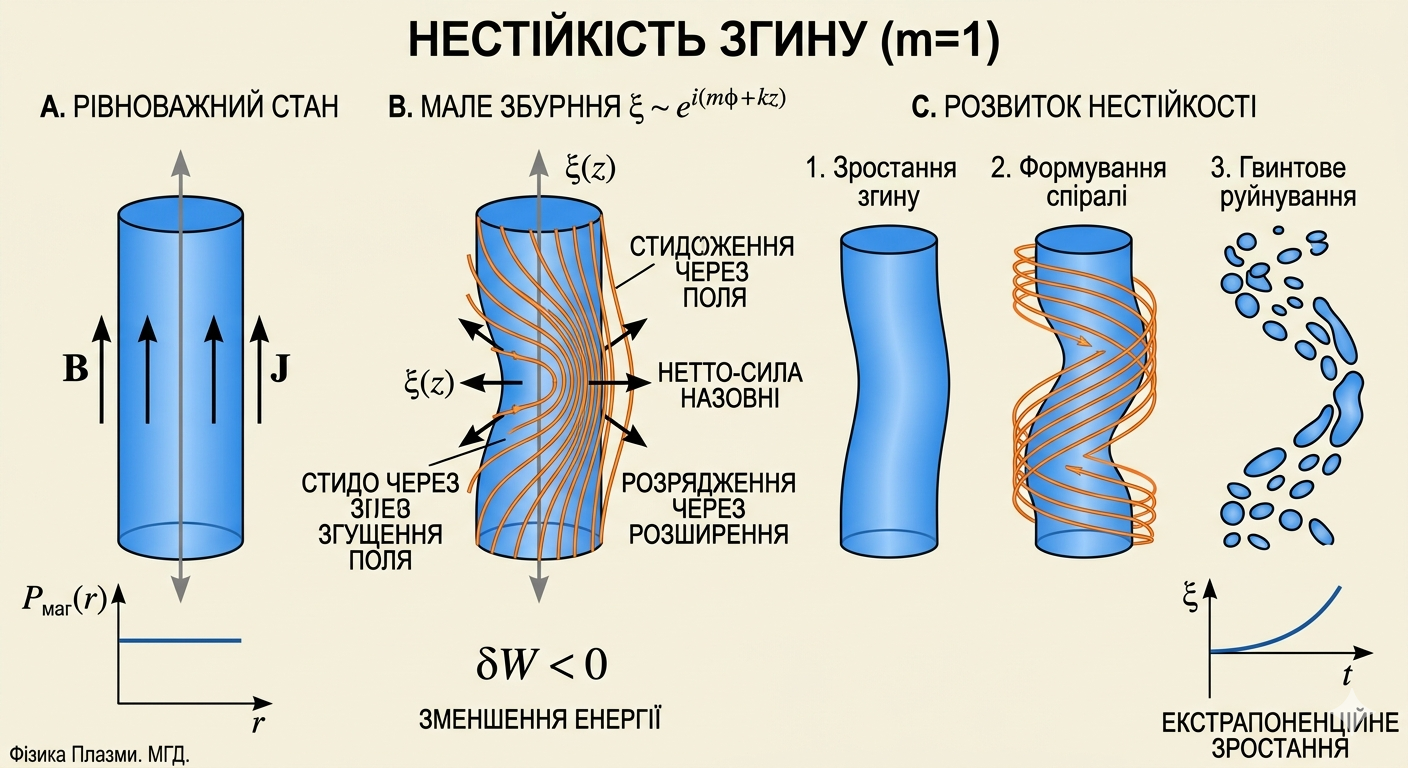
\includegraphics[width=0.75\linewidth]{pic/m1_instab.png}
\end{center}
%---------------------------------------------------------

\end{frame}

% --- Слайд 8: Енергетичний принцип (Детально) ---
\begin{frame}{Енергетичний принцип $\delta W$}{}
	\begin{block}{Варіація енергії}\justifying
		Робота, яку виконують сили при зміщенні $\vec{\xi}$:
		\begin{equation*}
			\delta W = -\frac{1}{2} \int \vec{\xi} \cdot \vec{F}(\vec{\xi}) \, dV
		\end{equation*}
	\end{block}
	\begin{itemize}
		\item Якщо для всіх можливих $\vec{\xi}$ виконується $\delta W > 0$, система \textbf{стійка}.
		\item Якщо існує хоча б одне зміщення, при якому $\delta W < 0$, система \textbf{нестійка}.
	\end{itemize}
	Це дозволяє аналізувати стійкість, не розв'язуючи рівняння руху.
\end{frame}

% --- Слайд 9: Стабілізація полем Bz ---
\begin{frame}{Стабілізація поздовжнім полем}{}
	\begin{block}{Ефект «магнітної пружини»}\justifying
		Якщо всередині плазми є поле $B_z$, то будь-яка деформація призводить до:
		\begin{enumerate}
			\item Стиснення ліній $B_z$ (при перетяжці $m=0$).
			\item Вигину ліній $B_z$ (при $m=1$).
		\end{enumerate}
	\end{block}
	Внаслідок вмороженості магнітне поле чинить опір деформації. Робота на деформацію поля $\delta W_{mag} > 0$ сприяє стабілізації.
\end{frame}

% --- Слайд 10: Критерій Крускала-Шафранова ---
\begin{frame}{Критерій Крускала-Шафранова}{}
	Для стійкості моди $m=1$ у токамаці (радіус $a$, великий радіус $R$) необхідне сильне поле $B_z$.
	\begin{exampleblock}{Запас стійкості}\justifying
		\begin{equation*}
			q(a) = \frac{a B_z}{R B_\phi} > 1
		\end{equation*}
	\end{exampleblock}
	Фізичний зміст: силова лінія має зробити принаймні один повний оберт вздовж тора, перш ніж зробить один оберт за кутом $\phi$. Це «заплутує» нестійкість.
\end{frame}

% --- Слайд 11: Желобкова нестійкість ---
\begin{frame}{Желобкова нестійкість та кривизна}{}
	\begin{block}{Обмінна нестійкість}\justifying
		Виникає, коли плазма і магнітне поле міняються місцями без деформації ліній (це мінімізує витрати енергії на деформацію поля).
	\end{block}
	Це стається в областях, де силові лінії \alert{опуклі} в бік плазми.

\end{frame}

% --- Слайд 12: Магнітний шир ---
\begin{frame}{Магнітний шир (Shear)}{}
	\begin{definition}
		\textbf{Шир} ($s$) --- це просторова зміна кута нахилу магнітних ліній: $s = \frac{r}{q} \frac{dq}{dr}$.
	\end{definition}
	\begin{itemize}
		\item Якщо $q$ змінюється з радіусом, збурення, яке «налаштоване» на резонанс з лініями поля в одному шарі, виходить з резонансу в сусідньому.
		\item Шир «розриває» збурення, не даючи їм розвиватися.
	\end{itemize}
\end{frame}

% --- Слайд 13: Резистивні моди (Тиринг) ---
\begin{frame}{Неідеальна МГД: Тиринг-нестійкість}{}
	\begin{alertblock}{Вплив опору}\justifying
		Якщо провідність $\sigma$ скінченна, закон вмороженості порушується. Лінії поля можуть перезамикатися.
	\end{alertblock}
	\begin{itemize}
		\item Це призводить до утворення \textbf{магнітних островів}.
		\item Тиринг-нестійкість розвивається повільніше за ідеальні моди, але вона критична для утримання енергії в токамаках.
	\end{itemize}

\end{frame}

\end{document}